\documentclass[14pt,fleqn]{extarticle}
\RequirePackage{prepwell}

\newcommand\N{\mathbb{N}}
\newcommand\fx{9x^2+6x-5}
\newcommand\invfx{\frac{\sqrt{x+6} - 1}{3}}

\previewoff

\begin{document} 
\begin{question}
	\statement 

Let $f:\N\to\N$ be a function defined as $f(x) = \fx$. Show that 
$f:\N\to S$, where $S$ is the range of $f$ is invertible. Find the 
inverse of $f$ and hence find $f^{-1}(43)$ and $f^{-1}(163)$ 
      
      \begin{step}
  \begin{options} 
     \correct 
       
       The plot of $f(x)$ will be as shown below where the dotted line 
       is the parabolic curve $\fx$ 
       
       \begin{center}
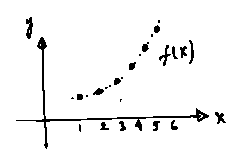
\includegraphics[scale=1.5]{1427-C.eps}
\end{center}
       
     \incorrect
     
     $f(x)$ will be a continuous parabolic curve as shown below 
     
     \begin{center}
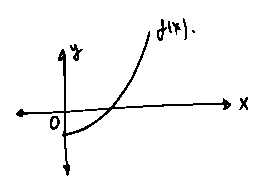
\includegraphics[scale=1.5]{1427-A.eps}
\end{center}
        
    \end{options} 
     \reason 
     
     $f(x) = f:\N\to\N$. Which means that $f(x)$ is defined \underline{only for $x\in\N$}\newline 
     
     Hence, $f(x)$ is defined for $x=1,2,3,\ldots\infty$. But it is not defined for $x=1.5$ or $x=100.4454$ because these numbers $\notin\N$\newline 
     
     Nor is $f(x)$ defined for $x=0$ as $0\notin\N$\newline 
     
     Notice also $f(2) > f(1), f(3) > f(2)$ and so on. Which means, $f(x)$ is strictly increasing in $\N$. Hence, it looks as below
     
     \begin{center}
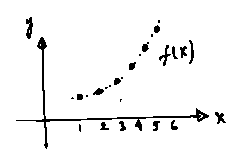
\includegraphics[scale=1.5]{1427-C.eps}
\end{center}

\underline{The dotted line is the parabola} $\fx$

\end{step}

\begin{step}
  \begin{options} 
     \correct 
       
     \begin{center}
  \begin{tabular}{lNN}
   \toprule
        Property & f(x)? & \text{Why?} \\
   \midrule 
   Injective & \checkmark & f(x)\neq f(y) \implies x\neq y \\
    \midrule 
    Surjective & \checkmark & y\in S\implies x\in\N \\
    \bottomrule
  \end{tabular}
\end{center} 
    
    And hence, $f(x)$ is also \underline{bijective/invertible}
        
    \end{options} 
     \reason 
     
     We haven't found the co-domain $S$ mentioned in the question. 
     But even then, just by looking at the plot of $f(x)$, we can 
     say that $f(x)$ is 
     
     \begin{center}
  \begin{tabular}{lNl}
   \toprule
        & \text{Why?} & Also called \\
   \midrule 
   1-to-1 & x\neq y \implies f(x)\neq f(y) & Injective \\
    \midrule 
    Onto & \text{For every }y\in S,\text{ there is a }x\in\N & Surjective \\
    \bottomrule
  \end{tabular}
\end{center}

And as $f(x)$ is \underline{both 1-to-1 and onto}, it is therefore also 
\underline{invertible (bijective)}
\end{step}

\begin{step}
  \begin{options} 
     \correct 
       
       \begin{align}
       y &= \fx \\
       \therefore x &= \frac{1}{3} \left[\sqrt{y + 6} - 1 \right] \\[5pt]
       \implies f^{-1}(x) &= \invfx \\[10pt]
       \text{Hence }f^{-1}(43) &= 2\text{ and } f^{-1}(163) = 4 
\end{align}
     \incorrect
     
     \begin{align}
       y &= \fx \\
       \therefore x &= \frac{1}{3} \left[\sqrt{y + 9} - 2 \right] \\[5pt]
       \implies f^{-1}(x) &= \dfrac{\sqrt{x+9} - 2}{3} \\[10pt]
       \text{Hence }f^{-1}(43) &= \dfrac{\sqrt{52}-2}{3}\\[5pt]
       \text{ and } f^{-1}(163) &= \dfrac{\sqrt{172}-2}{3}
\end{align}
        
    \end{options} 
     \reason 
     
     If $f:\N\to S$, then $f^{-1}:S\to\N$. Which means, that the output of $f^{-1}(x)$ will be a natural number \newline 
     
     That said, 
     \begin{align}
     y &= \fx = \left\lbrace (3x+1)^2 - 1\right\rbrace -5 \\[-10pt]
     &= (3x+1)^2 - 6 \\[10pt]
     \therefore x &= \dfrac{\sqrt{y+6}-1}{3} 
\end{align}

In the last equation, we evaluate $x$ in terms of $y$. Hence, $x$ is the \underline{dependent} variable and $y$ is the \underline{independent} variable\newline 

And by convention, we use $x$ for independent and $y$ for dependent variables\newline 

Hence, 
\[ x = \frac{\sqrt{y+6}-1}{3} \implies f^{-1}(x) = \frac{\sqrt{x+6}-1}{3} \]

And therefore, 
\begin{align}
f^{-1}(43) &= \frac{\sqrt{43+6}-1}{3} = 2 \\[5pt]
f^{-1}(163) &= \frac{\sqrt{163+6}-1}{3} = 4 
\end{align}
\end{step}
\end{question} 
\end{document} 